\section{A Model Problem}
\label{sec:ginzburg_landau}

The asymptotic center-manifold derived in section~\ref{sec:center_manifold_derivation} is applied to a Ginzburg-Landau model which is described by a complex-conjugate pair of equations as,
\begin{subequations}
	\label{eqn:ginzburg_landau}
	\begin{align}
		\dfrac{\partial A}{\partial t} =& \left[\delta_{1}\nabla + \delta_{2} + \delta_{3}x + \delta_{4}\Lap\right]A + \delta_{5}|A|^{2}A, \\
		%
		\dfrac{\partial A^{*}}{\partial t} =& \left[\delta^{*}_{1}\nabla + \delta^{*}_{2} + \delta^{*}_{3}x + \delta^{*}_{4}\Lap\right]A^{*} + \delta^{*}_{5}|A|^{2}A^{*}. 
	\end{align}
\end{subequations}
Where, $x$ is the spatial coordinate, $\nabla$ and $\Lap$ are the one-dimensional gradient and Laplacian operators, and the superscript $^{*}$ represents complex conjugation. Typically such a model would arise as the simplified dynamics of a more detailed dynamical system. Here the Ginzburg-Landau model itself is treated as the underlying dynamical model. Such models have often been utilized to investigate local and global bifurcations in spatially developing flows \citep{chomaz88,chomaz05}. For $A=0$ at the left and right domain boundaries, it is easily seen that $A(x)=0$ represents a fixed point of the system, with the linear operators given by
\begin{align}
	\mathcal{L}_{0}	=& \left[\delta_{1}\nabla + \delta_{2} + \delta_{3}x + \delta_{4}\Lap\right], \nonumber \\
	%
	\mathcal{L}^{*}_{0} =&\left[\delta^{*}_{1}\nabla + \delta^{*}_{2} + \delta^{*}_{3}x + \delta^{*}_{4}\Lap\right], \nonumber
\end{align}
and the linear operator for both $A$ and $A^{*}$ written together as
\begin{eqnarray}
	\mathcal{L} = \begin{bmatrix}
		\mathcal{L}_{0}		& 0 \\
		0								  & \mathcal{L}^{*}_{0}
	\end{bmatrix}
\end{eqnarray}

For semi-infinite domains, $x\in[0,\infty)$, the spectrum for $\mathcal{L}_{1}$ is known analytically \citep{chomaz88} and is given by,
%\begin{subequations}
	\begin{align}
		\omega_{n}	=& \delta_{2} - \dfrac{\delta_{1}^{2}}{4\delta_{4}} + (\delta_{4}\delta_{3}^{2})^{1/3}\zeta_{n}, \label{eqn:eigenvalues} 
		%
		%\phi_{n}(x)		=& \mathrm{Ai}([-\delta_{3}/\delta_{4}]^{1/3}x + \zeta_{n}), \label{eqn:eigenvectors}
	\end{align}
%\end{subequations}
and the corrresponding complex conjugate for $\mathcal{L}^{*}_{0}$. Here $\mathrm{Ai}$ denotes the Airy function and $\zeta_{n}$ its countable set of zeros.
 The system parameters at bifurcation are chosen \emph{ad hoc} as $\delta^{0}_{1} = -1.0$, $\delta^{0}_{2} = 0.741 + 1.025i$, $\delta^{0}_{3}=-0.125$, $\delta^{0}_{4}=(1.0 - i)/\sqrt{2}$ and $\delta^{0}_{5} =-0.1+0.1i$, which results in a single critical eigenmode with eigenvalue $\omega_{c} = 1.0i$ for $\mathcal{L}_{0}$ and its conjugate, $-1.0i$ for $\mathcal{L}^{*}_{0}$, and all other eigenvalues have negative real parts. 
 
 A center-manifold approximation of the model problem requires the evaluation of restricted resolvents, which is a difficult problem to solve analytically. Therefore the problem is considered in a trucated domain of $x\in [0,40]$ with the boundary conditions of $A = 0$ at $x=0$ and, $\partial A/\partial x = 0$ at $x=40$. Due to the spatially localized nature of the first few eigenvectors (which dictate the global dynamics), this truncation does not affect the dynamics in any significant manner, as can be seen from the comparison of the numerically evaluated spectrum in the truncated domain to the analytical spectrum in the semi-infinite domain (figure~\ref{fig:GL_spectrum}). The numerical spectrum was obtained via the implicitly restarted Arnoldi method \citep{sorensen92}.
\begin{figure}
	\centering
	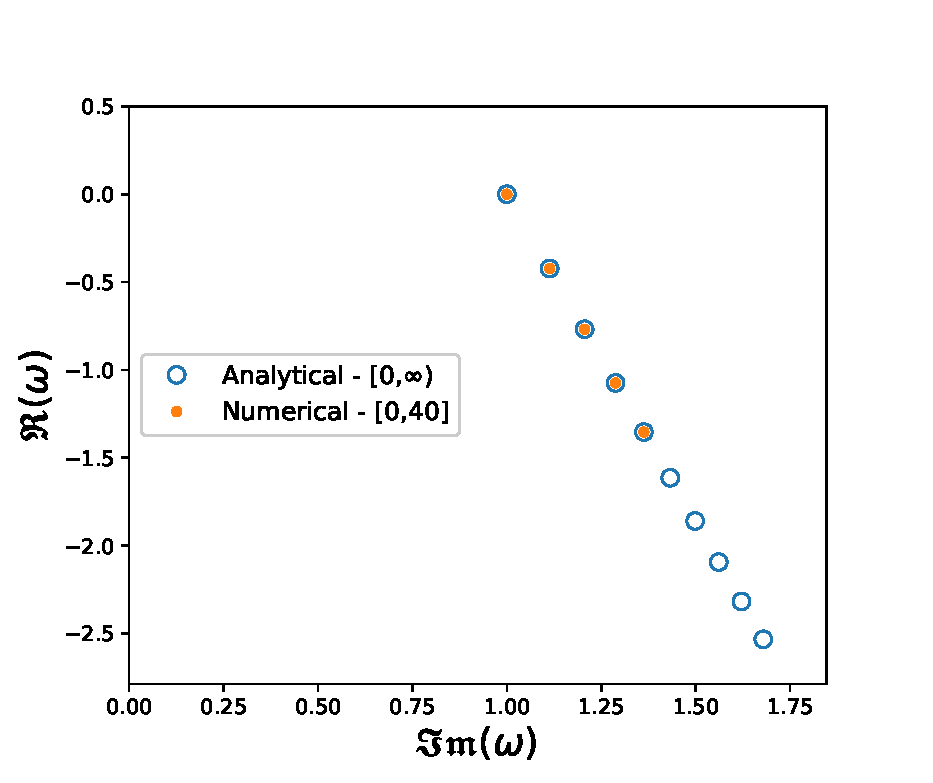
\includegraphics[width=0.49\textwidth]{GL_spectra}
	\caption{Comparison of the numerically evaluated spectrum of the Ginzburg-Landau model $(\mathcal{L}_{0})$ in the truncated domain with the analytical spectrum in the semi-infinite domain.}
	\label{fig:GL_spectrum}
\end{figure}

The structure of the eigenmodes is given by,
 \begin{align}
	\vecv_{5} = \begin{Bmatrix}
		\phi_{c} \\
		0 
	\end{Bmatrix}, & \hspace{2mm}
	%
	\vecv_{6} = \begin{Bmatrix}
		0 \\
		\phi^{*}_{c} 
	\end{Bmatrix}, \nonumber
\end{align}
where, $(\omega_{c},\phi_{c})$ and $(\omega^{*}_{c},\phi^{*}_{c})$ are the critical eigenpairs of $\mathcal{L}_{0}$ and $\mathcal{L}^{*}_{0}$ respectively. Similarly, the adjoint eigenmodes are denoted as,
\begin{align}
	\vecw_{5} = \begin{Bmatrix}
		\chi_{c} \\
		0 
	\end{Bmatrix}, & \hspace{2mm}
	%
	\vecw_{6} = \begin{Bmatrix}
		0 \\
		\chi^{*}_{c} 
	\end{Bmatrix}, \nonumber
\end{align}
where, $(\omega^{*}_{c},\chi_{c})$ and $(\omega_{c},\chi^{*}_{c})$ are the eigenpairs of corresponding adjoint linear operators $\mathcal{L}^{\dagger}_{0}$ and $\mathcal{L}^{*\dagger}_{0}$ respectively. The numerically calculated eigenvectors $\phi_{c}$ and $\chi_{c}$ are shown in figure~\ref{fig:GL_fields}. The projection operator into the stable subspace of $\mathcal{L}$ is defined as
\begin{align}
	\mathbf{Q} = \mathbf{I} - \vecv_{5}\vecw_{5}^{H} - \vecv_{6}\vecw_{6}^{H}. \nonumber
\end{align}
The projectors into the stable subspaces of $\mathcal{L}_{0}$ and $\mathcal{L}^{*}_{0}$ are denoted as $\mathbf{Q}_{0}$ and $\mathbf{Q}^{*}_{0}$, and are given by,
\begin{align}
	\mathbf{Q}_{0} 			=& \mathbf{I} - \phi_{c}\chi^{H}_{c}, & 
	\mathbf{Q}^{*}_{0} 	=& \mathbf{I} - \phi^{*}_{c}\chi^{*H}_{c}. \nonumber
\end{align}

The system in equation~\eqref{eqn:ginzburg_landau} has a total of five parameters (ten including the complex-conjugate pairs) that can be varied from their bifurcation values. In order to avoid an explosion in the number of terms $T_{k}$ arising from the combinatorial problem, only the variations in $\delta_{3},\delta_{4},\delta^{*}_{3}$ and $\delta^{*}_{4}$ are considered, which suffice to illustrate the derivation of the asymptotic center-manifold under parameter variations. Although the parameters are complex-conjugate pairs, it turns out to be simplest to treat them all as independent parameters and enforce the complex-conjugate property later when parameter values are prescribed, which is essentially the same as treating $A$ and $A^{*}$ independently and having two independent critical eigenvectors $\vecv_{5}$ and $\vecv_{6}$. 
The extended variable for the parameter evolution is then $\vecnu = [\delta'_{3};\delta'_{4};\delta'^{*}_{3};\delta'^{*}_{4}]$, with 
\begin{align}
	\delta_{3} =& \delta^{0}_{3} + \delta'_{3},& \delta_{4} =& \delta^{0}_{4} + \delta'_{4}, \nonumber \\
	\delta^{*}_{3} =& (\delta^{0}_{3})^{*} + \delta'^{*}_{3}, &\delta^{*}_{4} =& (\delta^{0}_{4})^{*} + \delta'^{*}_{4}. \nonumber
\end{align}
The extended state vector is denoted as $\widehat{A} = [A; A^{*}; \vecnu]$. With the knowledge of the linear operator and having calculated the critical eigenmodes, all the terms for the center-manifold approximation can now be easily built. 
The extended linear operator is given by,
 \begin{align}
 	\mathcal{\widehat{L}} = \begin{bmatrix}
 		\mathcal{L}_{0} 	   & 0											&	0 \\
 		0									  & \mathcal{L}^{*}_{0}		&   0 \\
 		0									  & 0											&  0
 	\end{bmatrix}. \nonumber
 \end{align}
This results in six critical modes for the extended system - two critical modes resulting from the original linear system $\mathcal{L}$ and four parameter modes due to system extension. The direct and adjoint eigenvector matrices are given by
 \begin{align}
 	\mathbf{\widehat{V}} =& [\efield{v}_{1};\efield{v}_{2};\efield{v}_{3};\efield{v}_{4};\efield{v}_{5};\efield{v}_{6}] =&
 	\begin{bmatrix}
        0 	    	      &  0		            &  0              &  0              &  \phi_{c} &  0              \\
        0		      &  0		            &  0              &  0              &  0        &  \phi^{*}_{c}   \\
 	  \vfield{e}_{1}  &  \vfield{e}_{2}       &  \vfield{e}_{3} &  \vfield{e}_{4} &  0        &  0              \\
 	\end{bmatrix}, \nonumber \\
 	%
 	\mathbf{\widehat{W}} =&
 	[\efield{w}_{1};\efield{w}_{2};\efield{w}_{3};\efield{w}_{4};\efield{w}_{5};\efield{w}_{6}] =&
 	\begin{bmatrix}
        0 	    	      &  0		            &  0              &  0              &  \chi_{c} &  0              \\
        0		      &  0		            &  0              &  0              &  0        &  \chi^{*}_{c}   \\
 	  \vfield{e}_{1}  &  \vfield{e}_{2}       &  \vfield{e}_{3} &  \vfield{e}_{4} &  0        &  0              \\
 	\end{bmatrix}. \nonumber
 \end{align}
resulting in the reduced system matrix,
\begin{align}
	\mathbf{\widehat{K}} = \begin{bmatrix}
		0 & 0 & 0 & 0 & 0& 0 \\ 
		0 & 0 & 0 & 0 & 0& 0 \\ 
		0 & 0 & 0 & 0 & 0& 0 \\ 
		0 & 0 & 0 & 0 & 0& 0 \\ 
		0 & 0 & 0 & 0 & \omega_{c} & 0 \\ 
		0 & 0 & 0 & 0 & 0 & \omega^{*}_{c}
	\end{bmatrix}. \nonumber
\end{align}
Due to the absence of purely real critical eigenvalues in the original system, the $\Gammabf$ matrix vanishes. 

To avoid confusion with the spatial variable $x$, the critical mode amplitudes are denoted by $\zbf = [z_{1};z_{2};z_{3};z_{4};z_{5};z_{6}]$, the stable component solution of the original system is given by $A_{s} = [A_{1s}; A_{2s}]$, and in the extended space it is $\widehat{A}_{s} = [A_{1s}; A_{2s}; 0]$. Thus the total solution is written as,
\begin{eqnarray}
	\widehat{A} = \widehat{\mathbf{V}}\zbf + \widehat{A}_{s}. \nonumber
\end{eqnarray}
The non-linear term of the original system is given by $\mathcal{N}_{NL} =  [\mathcal{N}_{1}; \mathcal{N}_{2}]$, with $\mathcal{N}_{1}$ and $\mathcal{N}_{2}$ defined as, 
\begin{align}
 	\begin{split}
 		\mathcal{N}_{1} =&
			z_{1}z_{5}x\phi_{c} + z_{1}xA_{1s} + z_{2}z_{5}\Lap\phi_{c} + z_{2}\Lap A_{1s} \\
			%
			 &+ \delta^{0}_{5}(\phi^{*}_{c}z_{6} +  A_{2s}) (\phi_{c}z_{5} +  A_{1s})(\phi_{c}z_{5} +  A_{1s}),
	\end{split} \nonumber \\
	%
	\begin{split}
		\mathcal{N}_{2} =&
		z_{3}z_{6}x\phi^{*}_{c} + z_{3}xA_{2s} + z_{4}z_{6}\Lap\phi^{*}_{c} + z_{4}\Lap A_{2s} \\
		%
		&+ \delta^{0*}_{5}(\phi_{c}z_{5} +  A_{1s}) (\phi^{*}_{c}z_{6} +  A_{2s})(\phi^{*}_{c}z_{6} +  A_{2s}),
	\end{split} \nonumber
\end{align}
and in the extended space it is defined as $\mathcal{\widehat{N}}_{NL} =  [\mathcal{N}_{1}; \mathcal{N}_{2}; 0]$. The evolution equations for the critical and stable subspaces are
\begin{subequations}
	\label{eqn:GL_canonical}
\begin{align}
	\dfrac{d z_{i}}{dt}	=& 0, \hspace{10mm} \text{for } i \in {1,2,3,4},\\
	%
	\dfrac{d z_{5}}{dt}	=& \omega_{c}z_{5} + \chi_{c}^{H}\mathcal{N}_{1},  \\
	%
	\dfrac{d z_{6}}{dt}	=& \omega^{*}_{c}z_{6} + \chi^{*H}_{c}\mathcal{N}_{2},  \\
	\dfrac{\partial A_{s}}{\partial t} =& \mathbf{Q}\mathcal{L}\mathbf{Q}A_{s} + \mathbf{Q}\mathcal{N}_{NL}.
\end{align}
\end{subequations}
The center-manifold theorem is applied to equation~\eqref{eqn:GL_canonical} and the stable component solution are evaluated asympotically as a power series in $\zbf$, 
\begin{align}
	\label{eqn:GL_asymptotic}
		\mathfrak{h}(\mathbf{z}) =& \sum_{a=1}^{6}\sum_{b=a}^{6} z_{a}z_{b}\vfield{y}_{a,b}
		 + \mathcal{O}(\mathbf{z}^{3}), \nonumber \\
		 %
		 \vfield{y}_{a,b} =& \begin{Bmatrix}
		 	\vfield{y}^{1}_{a,b} \vspace{1mm} \\
		 	\vfield{y}^{2}_{a,b}
		 \end{Bmatrix}.	\nonumber
\end{align}
For $M=6$, a total of $T_{2}=21$ terms are obtained at second order for the asymptotic approximation. All coupling terms $\vecg^{c}_{\alpha,\beta}$ vanish identically and only the following nontrivial forcing terms $\vecg_{\alpha,\beta}$ are obtained at second order,
%\begin{align}
%	\vecg_{1,1}  = \vecg_{1,2} = \vecg_{1,3}  = \vecg_{1,4} = \vecg_{1,6} = \vfield{0}, \nonumber \\
%	\vecg_{2,2} = \vecg_{2,3} = \vecg_{2,4} = \vecg_{2,6} = \vfield{0}, \nonumber \\
%	\vecg_{3,3} = \vecg_{3,4} = \vecg_{3,5} = \vfield{0}, \nonumber \\
%	\vecg_{4,4} = \vecg_{4,5} = \vfield{0}, \nonumber \\
%	\vecg_{5,5} = \vecg_{5,6} = \vecg_{6,6} = \vfield{0}, \nonumber
%\end{align}
%and,
\begin{align}
	\vecg_{1,5} =& 	\mathbf{Q}\cdot x\vecv_{5} =&
	\begin{Bmatrix}
		\mathbf{Q}_{0}x\phi_{c} \\
		0
	\end{Bmatrix}, \nonumber \\
	%
	\vecg_{2,5} =& 	\mathbf{Q}\cdot \Lap\vecv_{5} =&
	\begin{Bmatrix}
		\mathbf{Q}_{0}\Lap\phi_{c}	\\
		0
	\end{Bmatrix}, \nonumber \\
	%
	\vecg_{3,6} =& 	\mathbf{Q}\cdot x\vecv_{6} =&
	\begin{Bmatrix}
		0	\\
		\mathbf{Q}^{*}_{0}x\phi^{*}_{c}
	\end{Bmatrix}, \nonumber \\
	%
	\vecg_{4,6} =& 	\mathbf{Q}\cdot \Lap\vecv_{6} =&
	\begin{Bmatrix}
		0	\\
		\mathbf{Q}^{*}_{0}\Lap\phi^{*}_{c}
	\end{Bmatrix}, \nonumber
\end{align}
with all other forcing terms $\vecg_{\alpha,\beta}$ vanishing identically. This leads to the restricted resolvent solutions $\vecy_{\alpha,\beta}$ that satisfy,
 \begin{subequations}
 	\label{eqn:GL_resolvents}
	 \begin{align}
	 	\mathbf{Q}[(0 + \omega_{c})\mathbf{I} - \mathcal{L}]\mathbf{Q}\vecy_{1,5} =& \vecg_{1,5}, \\
	 	%
	 	\mathbf{Q}[(0 + \omega_{c})\mathbf{I} - \mathcal{L}]\mathbf{Q}\vecy_{2,5} =& \vecg_{2,5}, \\
	 	%
	 	\mathbf{Q}[(0 + \omega^{*}_{c})\mathbf{I} - \mathcal{L}]\mathbf{Q}\vecy_{3,6} =& \vecg_{3,6}, \\
	 	%
	 	\mathbf{Q}[(0 + \omega^{*}_{c})\mathbf{I} - \mathcal{L}]\mathbf{Q}\vecy_{4,6} =& \vecg_{4,6}, 
	 \end{align}
\end{subequations}
and all other second order terms $\vecy_{\alpha,\beta}$ vanishing identically. The resolvent solutions in terms of the individual fields are written as
 \begin{subequations}
 	\label{eqn:GL_sub_resolvents}
	 \begin{align}
	 	\mathbf{Q}_{0}[(0 + \omega_{c})\mathbf{I} - \mathcal{L}_{0}]\mathbf{Q}_{0}\vecy^{1}_{1,5} =& \mathbf{Q}_{0}x\phi_{c}, \\
	 	%
	 	\mathbf{Q}_{0}[(0 + \omega_{c})\mathbf{I} - \mathcal{L}_{0}]\mathbf{Q}_{0}\vecy^{1}_{2,5} =& \mathbf{Q}_{0}\Lap\phi_{c}, \\
	 	%
	 	%
	 	\mathbf{Q}^{*}_{0}[(0 + \omega^{*}_{c})\mathbf{I} - \mathcal{L}^{*}_{0}]\mathbf{Q}^{*}_{0}\vecy^{2}_{3,6} =& \mathbf{Q}^{*}_{0}x\phi^{*}_{c}, \\
		%
		\mathbf{Q}^{*}_{0}[(0 + \omega^{*}_{c})\mathbf{I} - \mathcal{L}^{*}_{0}]\mathbf{Q}^{*}_{0}\vecy^{2}_{2,5} =& \mathbf{Q}^{*}_{0}\Lap\phi^{*}_{c}.
		%
	 \end{align}
\end{subequations}
 Obviously, $\vecy^{2}_{1,5} = \vecy^{2}_{2,5} = \vecy^{1}_{3,6} = \vecy^{1}_{4,6} = 0$, with
 $\vecy^{2}_{3,6} = (\vecy^{1}_{1,5})^{*}$ and $\vecy^{2}_{4,6} = (\vecy^{1}_{2,5})^{*}$, as would be expected from the structure of the original equations. The second-order asymptotic fields $\vecy^{1}_{1,5}$ and $\vecy^{1}_{2,5}$ (along with the critical eigenvectors) are depicted in figure~\ref{fig:GL_fields}. The fields $\phi^{*}_{c}, \chi^{*}_{c},\vecy^{2}_{3,6}$ and $\vecy^{2}_{4,6}$ are the corresponding complex-conjugates (not shown). 
\begin{figure}
	\centering
	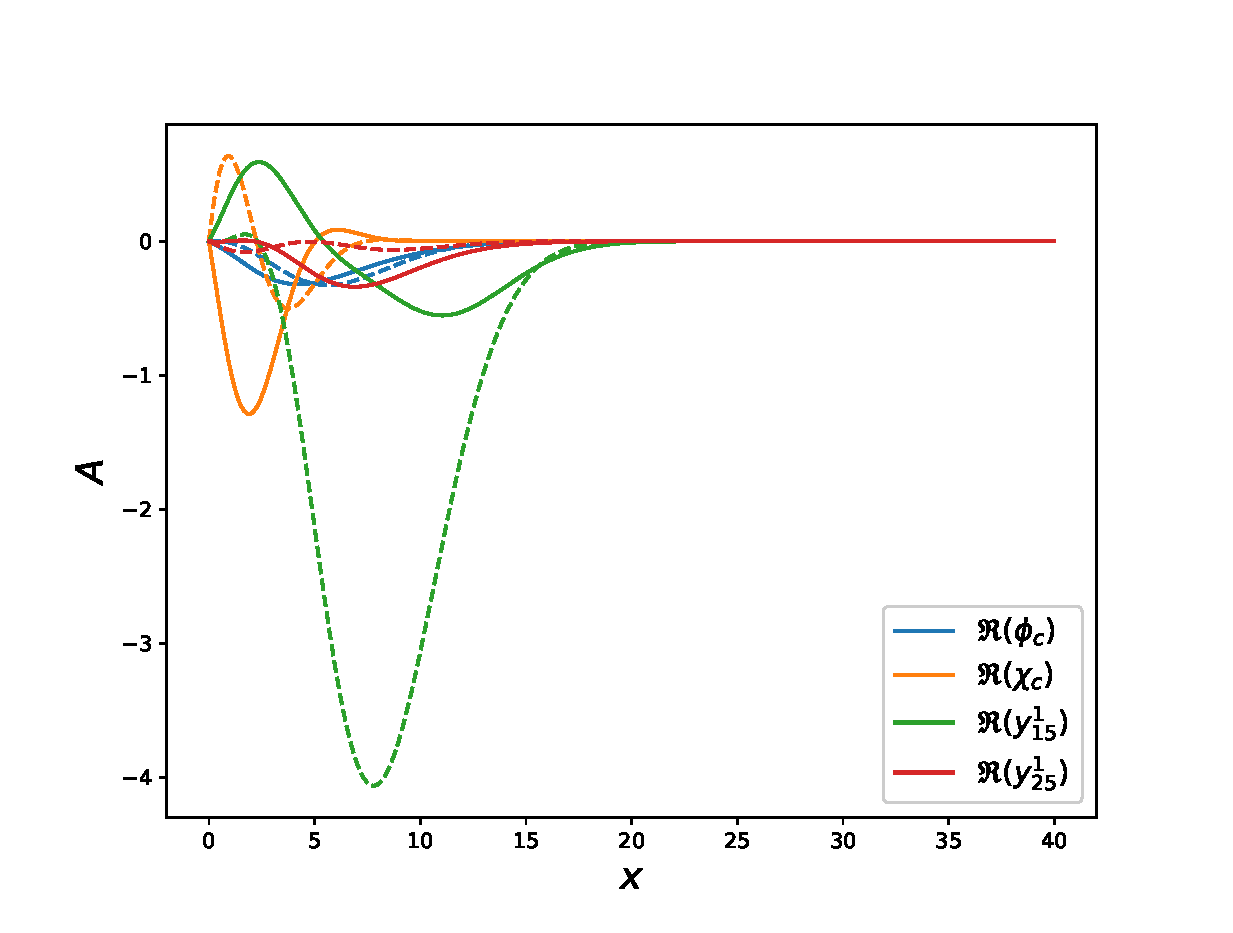
\includegraphics[width=0.49\textwidth]{GL_fields}
	\caption{Numerically evaluated eigenvector fields $\phi_{c}$ and $\chi_{c}$, along with the second-order approximations of stable components $\vecy_{1,5}$ and $\vecy_{2,5}$. The real pars of the fields depicted by solid lines while the imaginary parts are depicted with dashed lines of the same color.}
	\label{fig:GL_fields}
\end{figure} 

The complex-conjugation property may now be enforced so that $z_{6}=z^{*}_{5}, z_{3}=z^{*}_{1}, z_{4}=z^{*}_{2}$ and, the original parameter perturbations re-introduced, $z_{1} = \delta'_{3}, z_{2} = \delta'_{4}$. The resulting critical mode amplitude equation is
\begin{align}
	\label{eqn:stuart_landau}
	\begin{split}
	\dfrac{d z_{5}}{d t} =
	& \omega_{c}z_{5} + \delta'_{3}z_{5}(\chi^{H}_{c}x\phi_{c}) +  				(\delta'_{3})^{2}z_{5}(\chi^{H}_{c}x\vecy_{1,5}) \\
	%
	& + \delta'_{3}\delta'_{4}z_{5}(\chi^{H}_{c}x\vecy_{2,5}) + \delta'_{4}z_{5}(\chi^{H}_{c}\Lap\phi_{c}) \\
	%
	&  + \delta'_{3}\delta'_{4}z_{5}(\chi^{H}_{c}\Lap\vecy_{1,5}) + (\delta'_{4})^{2}z_{5}(\chi^{H}_{c}\Lap\vecy_{2,5}) \\
	%
	& + \delta^{0}_{5}|z_{5}|^{2}z_{5}(\chi^{H}_{c}|\phi_{c}|^{2}\phi_{c}),
	\end{split} 
\end{align}
and its complex conjugate for $z_{6}$, mirroring the original structure of equation~\eqref{eqn:ginzburg_landau}. In this case, the Ginzburg-Landau equation has been reduced to a Stuart-Landau like equation in the vicinity of the bifurcation point. The inner-products in equation~\eqref{eqn:stuart_landau} are evaluated numerically as,
\begin{align}
	\chi^{H}_{c}x\phi_{c} =&& 3.011 - 0.807i, \nonumber\\
	\chi^{H}_{c}x\vecy_{1,5} =&& 4.015 - 1.076i, \nonumber \\
	\chi^{H}_{c}x\vecy_{2,5} =&& -0.036 - 0.582i,  \nonumber \\
	\chi^{H}_{c}\Lap\phi_{c} =&& -0.169 + 0.153i, \nonumber \\
	\chi^{H}_{c}\Lap\vecy_{1,5} =&& 0.936 + 1.101i, \nonumber \\
	\chi^{H}_{c}\Lap\vecy_{2,5} =&& 0.194 - 0.114i, \nonumber \\
	\chi^{H}_{c}|\phi_{c}|^{2}\phi_{c} =&& 0.111 - 0.032i. \nonumber
\end{align}

The center-manifold reduction obtained in equation~\eqref{eqn:stuart_landau} can be compared with the original system by evaluating the angular frequencies obtained for the full system and its reduced counter part for parameter perturbations. The comparison is shown in figure~\ref{fig:omega_parameter_variation} for the variation of $\delta'_{3}$ and $\delta'_{4}$. The agreement is very good close to the bifurcation point with a systematic deviation arising at larger parameter variation, which would be expected given the asymptotic nature of the approximation. The deviation is also larger for $\delta'_{3}$ compared to $\delta'_{4}$, which could be qualitatively understood apriori, given the relatively large norm of $\vecy_{1,5}$, as seen in figure~\ref{fig:GL_fields}, which arises due to $\delta'_{3}$ perturbations. 
\begin{figure}
	\centering
	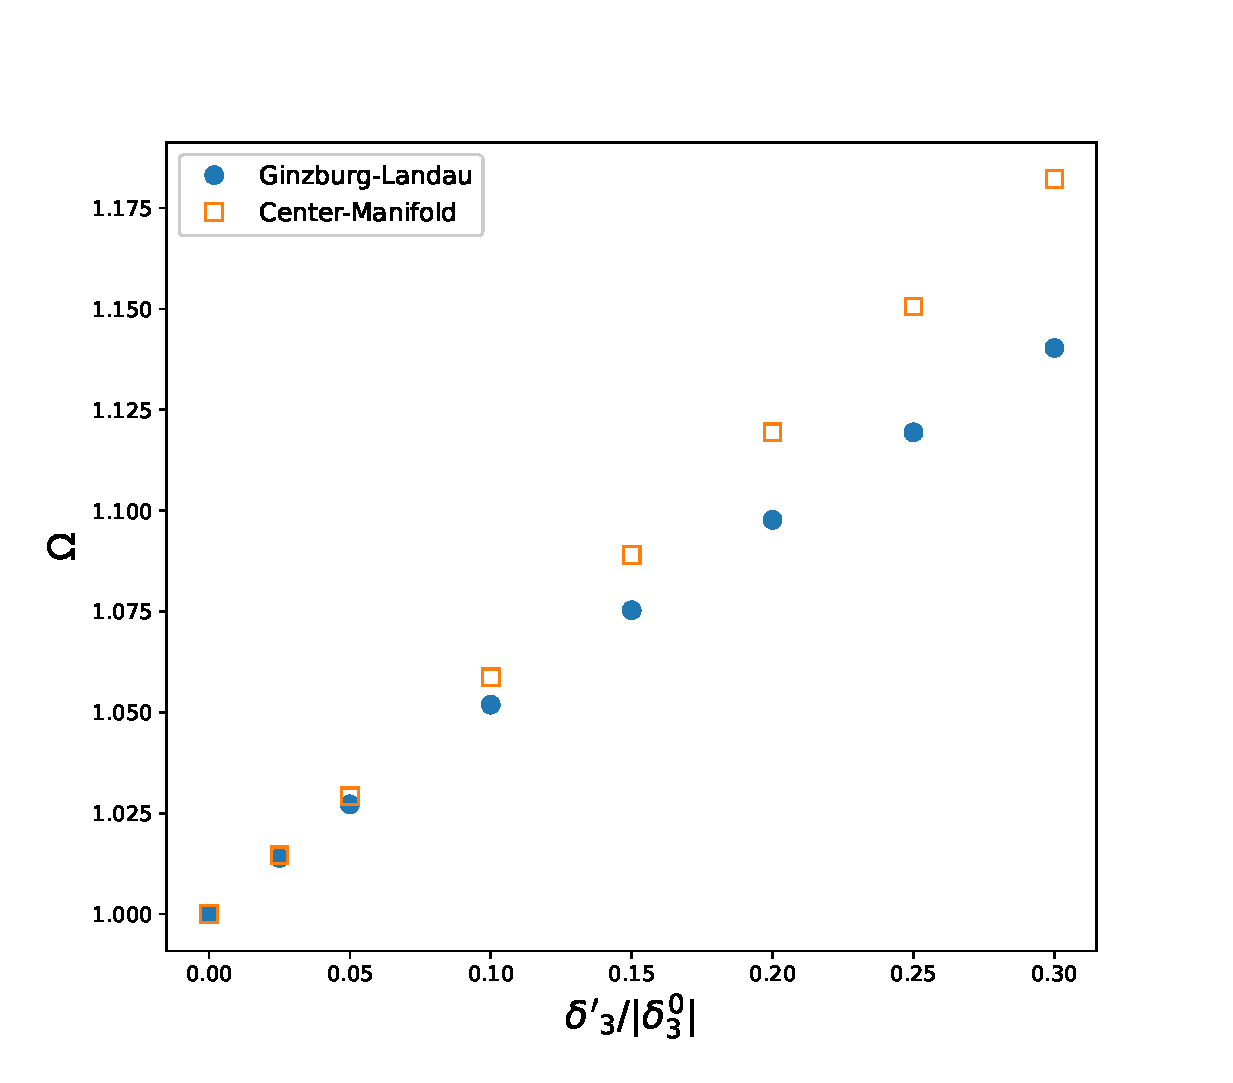
\includegraphics[width=0.49\textwidth]{center_manifold_omega1}
	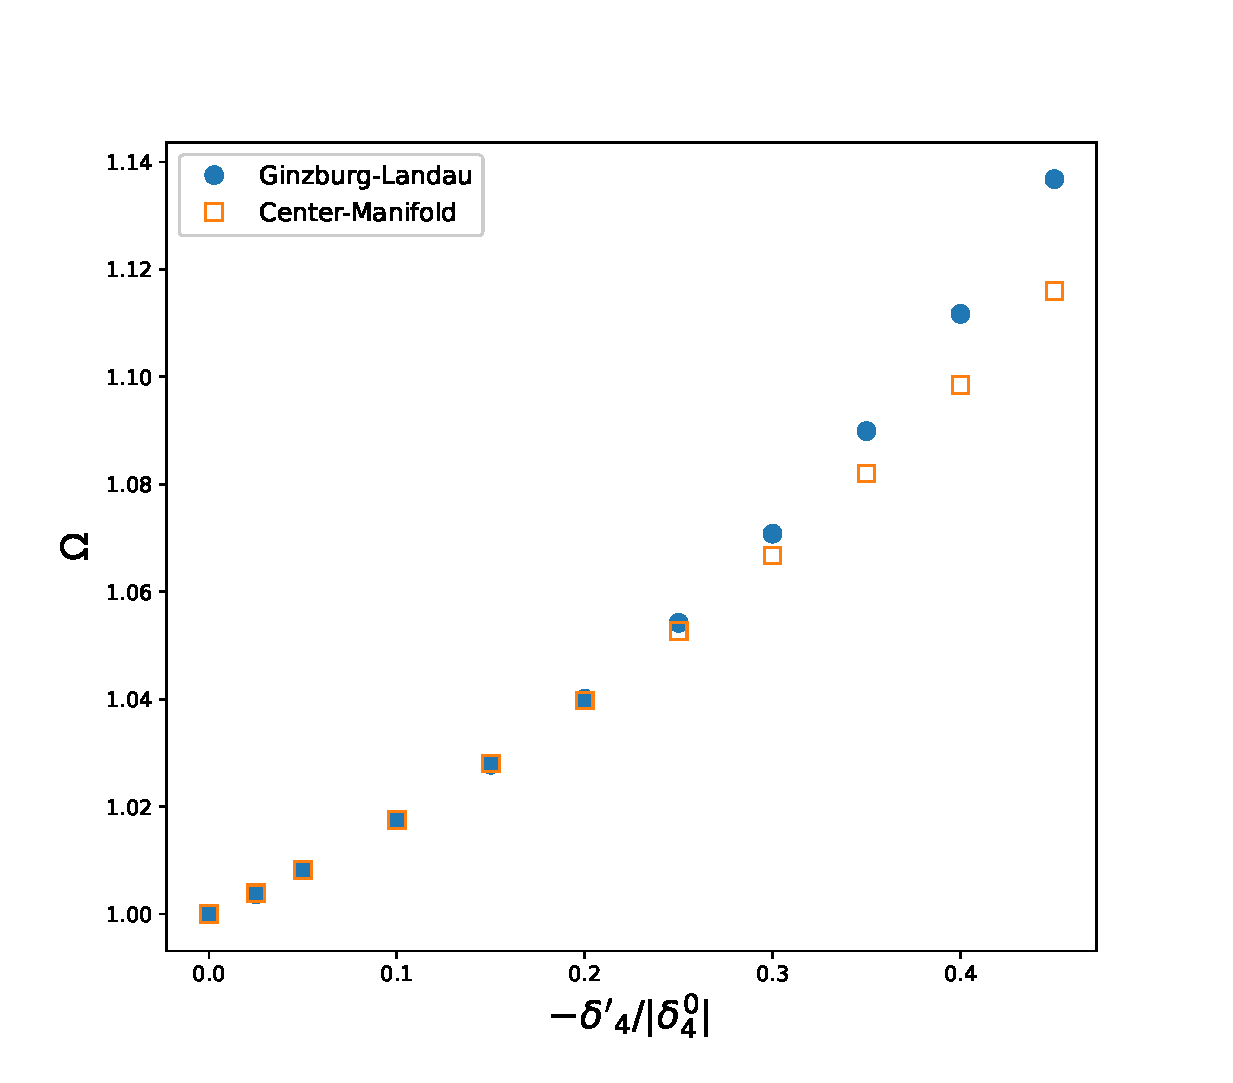
\includegraphics[width=0.49\textwidth]{center_manifold_omega2}
	\caption{Comparison of the angular frequencies obtained from the Ginzburg-Landau system, equation~\eqref{eqn:ginzburg_landau}, and its center-manifold reduction, equation~\eqref{eqn:stuart_landau} for different values of parameter perturbations. (Top) $\delta'_{4} = 0$ with varying $\delta'_{3}$ and, (bottom) $\delta'_{3} = 0$ with varying $\delta'_{4}$.}
	\label{fig:omega_parameter_variation}
\end{figure} 



